\documentclass[tikz,crop,convert={density=200,outext=.png},border=0.4cm]{standalone}

\usepackage{pgfplots}
\usepackage{amsmath}
\usetikzlibrary{arrows.meta}
\usepackage{physics}
\usepackage{xcolor}
\definecolor{mass_1}{RGB}{103,0,31}
\definecolor{mass_2}{RGB}{206,18,86}
\pgfplotsset{compat=newest,
    %width=6cm,
    %height=3cm,
    scale only axis=true,
    max space between ticks=25pt,
    try min ticks=5,
    every axis/.style={
        axis y line=middle,
        axis x line=middle,
        axis line style={thick,->,>=latex, shorten >=-.3cm}
    },
    every axis plot/.append style={thick},
    tick style={black, thick},
}
\tikzset{
    semithick/.style={line width=0.8pt},
}
\usepgfplotslibrary{groupplots}
\usepgfplotslibrary{dateplot}
% Document begins
\begin{document}
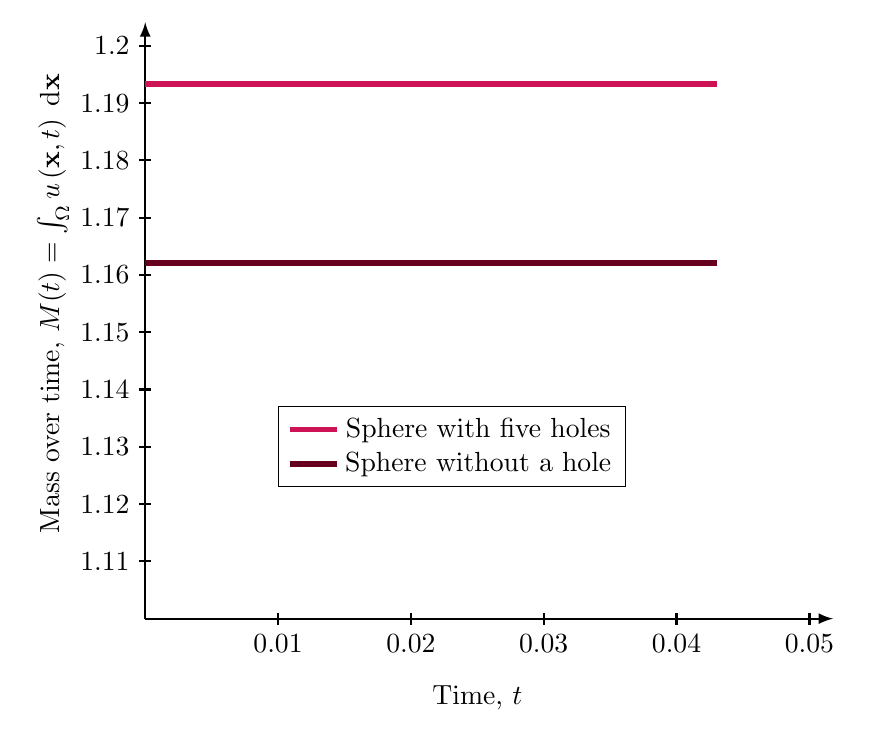
\begin{tikzpicture}
  % The axis of the plot
\begin{axis}[
    %title={Model: $\dv{y}{t}=\frac{2y}{t}$ with solution $y(t)=C_1t^2$\\Symmetry: $\Gamma_{\epsilon}=(t,y)\mapsto\left(\exp\left(\epsilon\right)t,\exp\left(-\epsilon\right)y\right)$},
    title style = {align=left},
    xlabel={Time, $t$},
    % ylabel={Incidence, $R(t)$},
    ylabel={Mass over time, $M(t)=\int_{\Omega}u\left(\mathbf{x},t\right)\;\dd\mathbf{x}$},        
    x label style={
      at={(axis description cs:0.5,-0.1)},
      anchor=north,
      /pgf/number format/.cd,
      fixed,
      fixed zerofill,
      %precision=2,
      /tikz/.cd      
    },
    y label style={
      at={(axis description cs:-0.1,0.55)},
      rotate=90,
      anchor=south,
    },    
    %xmin=0, xmax=82.5,
    xmin=0, xmax=0.05,
    ymin=1.1, ymax=1.2,
    %xtick={-30,-27,...,9},
    xtick={0.01,0.02,...,0.05},
    xticklabels = {$0.01$,$0.02$, $0.03$, $0.04$, $0.05$},
    %ytick={-15,-10,...,15},
    legend style={at={(axis description cs:0.2,0.3)},anchor=west},    
    %legend pos=north west,
    %ymajorgrids=true,
    grid style=dashed,
    scaled x ticks = false    
]
% Plot the model
\addplot[
color=mass_2,line width=2pt,
]
coordinates {%
(0.0,1.1933342220914462)
(2e-12,1.1933342221079917)
(4e-12,1.193334222111432)
(8e-12,1.1933342221125258)
(1.6e-11,1.1933342221177186)
(3.2e-11,1.1933342221081693)
(6.4e-11,1.193334222127259)
(1.28e-10,1.1933342221523044)
(2.56e-10,1.193334222163629)
(5.12e-10,1.1933342221482652)
(1.0239999999999998e-09,1.1933342221800975)
(2.0479999999999987e-09,1.1933342221999412)
(4.095999999999991e-09,1.193334222213344)
(8.191999999999929e-09,1.1933342222022634)
(1.6383999999999434e-08,1.1933342221673957)
(3.2767999999995466e-08,1.1933342221466074)
(6.553599999996372e-08,1.1933342221596241)
(1.3107199999970976e-07,1.1933342221863374)
(2.621439999976783e-07,1.1933342221849947)
(5.242879999814343e-07,1.193334222167068)
(1.0485759998516102e-06,1.1933342221728147)
(2.0971519988150635e-06,1.193334222181967)
(4.194303990555173e-06,1.1933342221785228)
(8.38860792498753e-06,1.193334222179295)
(1.6777215408376973e-05,1.1933342221786243)
(3.3554427394949846e-05,1.1933342221786845)
(6.710882899600741e-05,1.1933342221781444)
(0.00013421747222428296,1.1933342221781031)
(0.0002684336928032127,1.1933342221781018)
(0.0005184336928032127,1.1933342221781063)
(0.0007684336928032127,1.1933342221781031)
(0.0010184336928032128,1.1933342221781038)
(0.0012684336928032128,1.1933342221781076)
(0.0015184336928032128,1.193334222178108)
(0.0017684336928032128,1.1933342221781056)
(0.002018433692803213,1.1933342221781054)
(0.0022684336928032126,1.1933342221781107)
(0.002518433692803213,1.1933342221781098)
(0.002768433692803213,1.1933342221781074)
(0.0030184336928032133,1.1933342221781067)
(0.0032684336928032135,1.1933342221781076)
(0.0035184336928032137,1.19333422217811)
(0.003768433692803214,1.1933342221781116)
(0.004018433692803214,1.1933342221781111)
(0.004268433692803214,1.1933342221781134)
(0.004518433692803215,1.1933342221781114)
(0.004768433692803215,1.1933342221781107)
(0.005018433692803215,1.1933342221781116)
(0.005268433692803215,1.1933342221781111)
(0.0055184336928032155,1.1933342221781083)
(0.005768433692803216,1.1933342221781125)
(0.006018433692803216,1.1933342221781122)
(0.006268433692803216,1.1933342221781111)
(0.006518433692803216,1.193334222178115)
(0.006768433692803217,1.1933342221781158)
(0.007018433692803217,1.1933342221781125)
(0.007268433692803217,1.1933342221781165)
(0.007518433692803217,1.1933342221781162)
(0.0077684336928032175,1.1933342221781136)
(0.008018433692803218,1.1933342221781165)
(0.008268433692803218,1.193334222178116)
(0.008518433692803218,1.1933342221781156)
(0.008768433692803218,1.1933342221781196)
(0.009018433692803219,1.1933342221781167)
(0.009268433692803219,1.1933342221781162)
(0.009518433692803219,1.193334222178116)
(0.00976843369280322,1.1933342221781156)
(0.01001843369280322,1.1933342221781171)
(0.01026843369280322,1.1933342221781214)
(0.01051843369280322,1.1933342221781167)
(0.01076843369280322,1.193334222178122)
(0.01101843369280322,1.1933342221781176)
(0.01126843369280322,1.1933342221781202)
(0.01151843369280322,1.1933342221781233)
(0.011768433692803221,1.1933342221781196)
(0.012018433692803221,1.1933342221781225)
(0.012268433692803222,1.1933342221781298)
(0.012518433692803222,1.1933342221781267)
(0.012768433692803222,1.1933342221781191)
(0.013018433692803222,1.1933342221781262)
(0.013268433692803222,1.1933342221781307)
(0.013518433692803223,1.1933342221781258)
(0.013768433692803223,1.1933342221781247)
(0.014018433692803223,1.193334222178128)
(0.014268433692803223,1.1933342221781236)
(0.014518433692803224,1.1933342221781233)
(0.014768433692803224,1.1933342221781262)
(0.015018433692803224,1.193334222178128)
(0.015268433692803224,1.1933342221781227)
(0.015518433692803224,1.1933342221781282)
(0.015768433692803223,1.1933342221781287)
(0.016018433692803223,1.1933342221781262)
(0.016268433692803223,1.193334222178129)
(0.016518433692803224,1.1933342221781325)
(0.016768433692803224,1.1933342221781256)
(0.017018433692803224,1.193334222178127)
(0.017268433692803224,1.193334222178136)
(0.017518433692803224,1.1933342221781287)
(0.017768433692803225,1.1933342221781331)
(0.018018433692803225,1.1933342221781325)
(0.018268433692803225,1.1933342221781336)
(0.018518433692803225,1.1933342221781342)
(0.018768433692803226,1.1933342221781336)
(0.019018433692803226,1.1933342221781367)
(0.019268433692803226,1.1933342221781367)
(0.019518433692803226,1.1933342221781362)
(0.019768433692803226,1.1933342221781373)
(0.020018433692803227,1.1933342221781382)
(0.020268433692803227,1.1933342221781382)
(0.020518433692803227,1.1933342221781351)
(0.020768433692803227,1.193334222178135)
(0.021018433692803228,1.1933342221781342)
(0.021268433692803228,1.1933342221781347)
(0.021518433692803228,1.1933342221781373)
(0.021768433692803228,1.193334222178138)
(0.02201843369280323,1.1933342221781365)
(0.02226843369280323,1.1933342221781384)
(0.02251843369280323,1.1933342221781387)
(0.02276843369280323,1.1933342221781391)
(0.02301843369280323,1.1933342221781382)
(0.02326843369280323,1.1933342221781376)
(0.02351843369280323,1.1933342221781416)
(0.02376843369280323,1.1933342221781422)
(0.02401843369280323,1.19333422217815)
(0.02426843369280323,1.1933342221781416)
(0.02451843369280323,1.193334222178142)
(0.02476843369280323,1.193334222178143)
(0.02501843369280323,1.1933342221781413)
(0.02526843369280323,1.1933342221781424)
(0.02551843369280323,1.1933342221781489)
(0.025768433692803232,1.1933342221781436)
(0.026018433692803232,1.1933342221781469)
(0.026268433692803232,1.193334222178148)
(0.026518433692803232,1.1933342221781464)
(0.026768433692803233,1.1933342221781458)
(0.027018433692803233,1.193334222178148)
(0.027268433692803233,1.193334222178146)
(0.027518433692803233,1.1933342221781482)
(0.027768433692803234,1.1933342221781449)
(0.028018433692803234,1.1933342221781436)
(0.028268433692803234,1.1933342221781509)
(0.028518433692803234,1.1933342221781513)
(0.028768433692803234,1.1933342221781462)
(0.029018433692803235,1.193334222178151)
(0.029268433692803235,1.1933342221781458)
(0.029518433692803235,1.1933342221781558)
(0.029768433692803235,1.1933342221781496)
(0.030018433692803236,1.193334222178154)
(0.030268433692803236,1.1933342221781555)
(0.030518433692803236,1.1933342221781524)
(0.030768433692803236,1.1933342221781538)
(0.031018433692803236,1.1933342221781513)
(0.03126843369280324,1.1933342221781515)
(0.03151843369280324,1.1933342221781529)
(0.03176843369280324,1.193334222178153)
(0.03201843369280324,1.193334222178158)
(0.03226843369280324,1.193334222178154)
(0.03251843369280324,1.193334222178155)
(0.03276843369280324,1.1933342221781513)
(0.03301843369280324,1.1933342221781587)
(0.03326843369280324,1.1933342221781609)
(0.03351843369280324,1.1933342221781584)
(0.03376843369280324,1.1933342221781604)
(0.03401843369280324,1.1933342221781607)
(0.03426843369280324,1.193334222178163)
(0.03451843369280324,1.1933342221781558)
(0.03476843369280324,1.1933342221781624)
(0.03501843369280324,1.1933342221781595)
(0.03526843369280324,1.1933342221781644)
(0.03551843369280324,1.1933342221781695)
(0.03576843369280324,1.1933342221781609)
(0.03601843369280324,1.193334222178163)
(0.03626843369280324,1.1933342221781658)
(0.03651843369280324,1.1933342221781642)
(0.03676843369280324,1.1933342221781642)
(0.03701843369280324,1.1933342221781658)
(0.03726843369280324,1.1933342221781644)
(0.03751843369280324,1.1933342221781664)
(0.03776843369280324,1.1933342221781593)
(0.03801843369280324,1.1933342221781695)
(0.03826843369280324,1.193334222178172)
(0.03851843369280324,1.1933342221781722)
(0.03876843369280324,1.1933342221781702)
(0.039018433692803244,1.1933342221781678)
(0.039268433692803244,1.1933342221781658)
(0.039518433692803244,1.1933342221781675)
(0.039768433692803244,1.193334222178167)
(0.040018433692803244,1.1933342221781684)
(0.040268433692803245,1.1933342221781662)
(0.040518433692803245,1.1933342221781658)
(0.040768433692803245,1.1933342221781698)
(0.041018433692803245,1.1933342221781702)
(0.041268433692803246,1.1933342221781695)
(0.041518433692803246,1.1933342221781689)
(0.041768433692803246,1.193334222178174)
(0.042018433692803246,1.1933342221781698)
(0.042268433692803246,1.1933342221781775)
(0.04251843369280325,1.1933342221781749)
(0.04276843369280325,1.1933342221781715)
(0.04301843369280325,1.1933342221781744)
};
\addlegendentry{Sphere with five holes}

% Plot the data
\addplot[
color=mass_1,line width=2pt,
]
coordinates {%
(0.0,1.1621157751954196)
(2e-12,1.1621157751947375)
(4e-12,1.1621157751938178)
(8e-12,1.1621157751944085)
(1.6e-11,1.1621157751947593)
(3.2e-11,1.1621157751951243)
(6.4e-11,1.1621157751954085)
(1.28e-10,1.1621157751952422)
(2.56e-10,1.1621157751950757)
(5.12e-10,1.16211577519537)
(1.0239999999999998e-09,1.1621157751946563)
(2.0479999999999987e-09,1.162115775195037)
(4.095999999999991e-09,1.1621157751948883)
(8.191999999999932e-09,1.1621157751941762)
(1.6383999999999454e-08,1.162115775194627)
(3.27679999999956e-08,1.1621157751952642)
(6.553599999996471e-08,1.162115775194874)
(1.3107199999971767e-07,1.1621157751936408)
(2.62143999997742e-07,1.1621157751935305)
(5.242879999819492e-07,1.1621157751929667)
(1.0485759998558038e-06,1.1621157751930251)
(2.097151998849783e-06,1.1621157751928375)
(4.194303990851172e-06,1.162115775192268)
(8.388607927633172e-06,1.162115775192658)
(1.67772154335732e-05,1.1621157751918896)
(3.355442765009e-05,1.1621157751922)
(6.710883164520411e-05,1.1621157751922133)
(0.00013421749869027902,1.1621157751922186)
(0.00026843393190864763,1.1621157751922202)
(0.0005184339319086477,1.162115775192219)
(0.0007684339319086477,1.1621157751922173)
(0.0010184339319086477,1.1621157751922182)
(0.0012684339319086477,1.1621157751922229)
(0.0015184339319086477,1.162115775192225)
(0.0017684339319086477,1.1621157751922213)
(0.0020184339319086475,1.1621157751922204)
(0.0022684339319086477,1.1621157751922275)
(0.002518433931908648,1.1621157751922266)
(0.002768433931908648,1.1621157751922218)
(0.0030184339319086484,1.1621157751922273)
(0.0032684339319086486,1.1621157751922273)
(0.003518433931908649,1.1621157751922249)
(0.003768433931908649,1.162115775192227)
(0.004018433931908649,1.1621157751922244)
(0.0042684339319086495,1.1621157751922255)
(0.00451843393190865,1.1621157751922304)
(0.00476843393190865,1.162115775192224)
(0.00501843393190865,1.162115775192225)
(0.00526843393190865,1.1621157751922273)
(0.005518433931908651,1.162115775192226)
(0.005768433931908651,1.162115775192232)
(0.006018433931908651,1.1621157751922304)
(0.006268433931908651,1.1621157751922309)
(0.0065184339319086515,1.162115775192232)
(0.006768433931908652,1.162115775192235)
(0.007018433931908652,1.1621157751922315)
(0.007268433931908652,1.1621157751922326)
(0.007518433931908652,1.1621157751922315)
(0.007768433931908653,1.1621157751922384)
(0.008018433931908653,1.1621157751922364)
(0.008268433931908653,1.16211577519223)
(0.008518433931908653,1.1621157751922373)
(0.008768433931908654,1.1621157751922297)
(0.009018433931908654,1.1621157751922369)
(0.009268433931908654,1.1621157751922315)
(0.009518433931908654,1.1621157751922346)
(0.009768433931908654,1.1621157751922313)
(0.010018433931908655,1.1621157751922269)
(0.010268433931908655,1.1621157751922389)
(0.010518433931908655,1.162115775192233)
(0.010768433931908655,1.1621157751922337)
(0.011018433931908655,1.1621157751922369)
(0.011268433931908656,1.162115775192244)
(0.011518433931908656,1.1621157751922369)
(0.011768433931908656,1.162115775192239)
(0.012018433931908656,1.1621157751922464)
(0.012268433931908657,1.1621157751922346)
(0.012518433931908657,1.1621157751922397)
(0.012768433931908657,1.1621157751922464)
(0.013018433931908657,1.162115775192245)
(0.013268433931908657,1.1621157751922444)
(0.013518433931908658,1.1621157751922413)
(0.013768433931908658,1.1621157751922415)
(0.014018433931908658,1.1621157751922435)
(0.014268433931908658,1.1621157751922406)
(0.014518433931908659,1.1621157751922406)
(0.014768433931908659,1.1621157751922409)
(0.015018433931908659,1.1621157751922404)
(0.01526843393190866,1.16211577519224)
(0.01551843393190866,1.1621157751922429)
(0.01576843393190866,1.1621157751922422)
(0.01601843393190866,1.1621157751922417)
(0.01626843393190866,1.162115775192246)
(0.01651843393190866,1.1621157751922413)
(0.01676843393190866,1.1621157751922437)
(0.01701843393190866,1.1621157751922377)
(0.01726843393190866,1.1621157751922462)
(0.01751843393190866,1.1621157751922404)
(0.01776843393190866,1.1621157751922462)
(0.01801843393190866,1.1621157751922455)
(0.018268433931908662,1.162115775192241)
(0.018518433931908662,1.1621157751922435)
(0.018768433931908662,1.1621157751922477)
(0.019018433931908663,1.1621157751922475)
(0.019268433931908663,1.1621157751922475)
(0.019518433931908663,1.162115775192248)
(0.019768433931908663,1.1621157751922504)
(0.020018433931908663,1.1621157751922495)
(0.020268433931908664,1.1621157751922504)
(0.020518433931908664,1.162115775192247)
(0.020768433931908664,1.1621157751922515)
(0.021018433931908664,1.1621157751922526)
(0.021268433931908665,1.162115775192253)
(0.021518433931908665,1.162115775192252)
(0.021768433931908665,1.1621157751922484)
(0.022018433931908665,1.1621157751922544)
(0.022268433931908665,1.162115775192248)
(0.022518433931908666,1.162115775192254)
(0.022768433931908666,1.1621157751922493)
(0.023018433931908666,1.162115775192253)
(0.023268433931908666,1.1621157751922495)
(0.023518433931908667,1.162115775192254)
(0.023768433931908667,1.162115775192252)
(0.024018433931908667,1.1621157751922575)
(0.024268433931908667,1.1621157751922546)
(0.024518433931908667,1.1621157751922517)
(0.024768433931908668,1.1621157751922544)
(0.025018433931908668,1.162115775192255)
(0.025268433931908668,1.162115775192253)
(0.02551843393190867,1.1621157751922588)
(0.02576843393190867,1.162115775192252)
(0.02601843393190867,1.1621157751922504)
(0.02626843393190867,1.1621157751922582)
(0.02651843393190867,1.16211577519225)
(0.02676843393190867,1.162115775192261)
(0.02701843393190867,1.1621157751922626)
(0.02726843393190867,1.1621157751922615)
(0.02751843393190867,1.1621157751922557)
(0.02776843393190867,1.1621157751922522)
(0.02801843393190867,1.162115775192258)
(0.02826843393190867,1.1621157751922657)
(0.02851843393190867,1.162115775192262)
(0.02876843393190867,1.1621157751922635)
(0.02901843393190867,1.1621157751922617)
(0.02926843393190867,1.1621157751922608)
(0.029518433931908672,1.1621157751922644)
(0.029768433931908672,1.1621157751922624)
(0.030018433931908672,1.1621157751922664)
(0.030268433931908673,1.1621157751922664)
(0.030518433931908673,1.1621157751922662)
(0.030768433931908673,1.1621157751922664)
(0.031018433931908673,1.1621157751922626)
(0.031268433931908673,1.1621157751922624)
(0.031518433931908674,1.1621157751922673)
(0.031768433931908674,1.162115775192266)
(0.032018433931908674,1.162115775192266)
(0.032268433931908674,1.1621157751922653)
(0.032518433931908675,1.1621157751922697)
(0.032768433931908675,1.1621157751922677)
(0.033018433931908675,1.1621157751922626)
(0.033268433931908675,1.162115775192266)
(0.033518433931908675,1.1621157751922704)
(0.033768433931908676,1.1621157751922724)
(0.034018433931908676,1.1621157751922668)
(0.034268433931908676,1.1621157751922713)
(0.034518433931908676,1.1621157751922684)
(0.03476843393190868,1.1621157751922677)
(0.03501843393190868,1.162115775192274)
(0.03526843393190868,1.162115775192269)
(0.03551843393190868,1.1621157751922715)
(0.03576843393190868,1.1621157751922728)
(0.03601843393190868,1.162115775192276)
(0.03626843393190868,1.1621157751922786)
(0.03651843393190868,1.1621157751922742)
(0.03676843393190868,1.1621157751922742)
(0.03701843393190868,1.1621157751922768)
(0.03726843393190868,1.1621157751922726)
(0.03751843393190868,1.1621157751922808)
(0.03776843393190868,1.1621157751922706)
(0.03801843393190868,1.1621157751922784)
(0.03826843393190868,1.1621157751922735)
(0.03851843393190868,1.162115775192276)
(0.03876843393190868,1.1621157751922728)
(0.03901843393190868,1.162115775192278)
(0.03926843393190868,1.1621157751922842)
(0.03951843393190868,1.1621157751922786)
(0.03976843393190868,1.1621157751922815)
(0.04001843393190868,1.16211577519228)
(0.04026843393190868,1.1621157751922873)
(0.04051843393190868,1.1621157751922815)
(0.04076843393190868,1.1621157751922766)
(0.04101843393190868,1.1621157751922866)
(0.04126843393190868,1.1621157751922817)
(0.04151843393190868,1.162115775192284)
(0.04176843393190868,1.162115775192286)
(0.04201843393190868,1.1621157751922846)
(0.04226843393190868,1.1621157751922866)
(0.042518433931908683,1.162115775192289)
(0.042768433931908684,1.162115775192283)
(0.043018433931908684,1.1621157751922861)
};
\addlegendentry{Sphere without a hole}


\end{axis}
\end{tikzpicture}

\end{document}
